
%(BEGIN_QUESTION)
% Copyright 2007, Tony R. Kuphaldt, released under the Creative Commons Attribution License (v 1.0)
% This means you may do almost anything with this work of mine, so long as you give me proper credit

In this process, two chemical streams are mixed together in a reactor vessel.  The ensuing chemical reaction is exothermic (heat-producing) and must be cooled by a water cooling system to prevent overheating of the vessel and piping.  A temperature transmitter (TT) senses the reaction product temperature and sends a 4-20 mA signal to a temperature indicating controller (TIC).  The controller then sends a 4-20 mA control signal to the temperature valve (TV) to throttle cooling water flow:

$$\includegraphics[width=15.5cm]{i02931x01.eps}$$

Suppose an instrument technician adds a temperature-indicating chart recorder (TIR) to the temperature transmitter circuit, necessitating the addition of a 250 ohm resistor to the 4-20 mA circuit to provide a 1-5 volt voltage signal which the recorder can read.  Now the 4-20 mA temperature circuit has more resistance in it than it did before.

\vskip 10pt

Describe in detail the effect this circuit modification will have on the performance of the cooling system.

\underbar{file i02931}
%(END_QUESTION)





%(BEGIN_ANSWER)

This circuit modification will have absolutely no effect on the performance of the system, as long as the loop-powered transmitter receives its minimum terminal voltage for proper operation.

%(END_ANSWER)





%(BEGIN_NOTES)

Some students may think the additional 250 ohms will decrease current, resulting in a too-cool reading of temperature.  However, this is not how 4-20 mA current circuits work!

%INDEX% Basics, control loop troubleshooting: determining effect of specified fault(s)

%(END_NOTES)


